\graphicspath{{members/ssr/figures/}}

\subsubsection*{Plant Model}

Based on the physiological description of tomato plants - as provided by the user view - a plant model has
been chosen as shown by figure \ref{fig:plant:model:2}.

\begin{figure}[H]
    \centering
    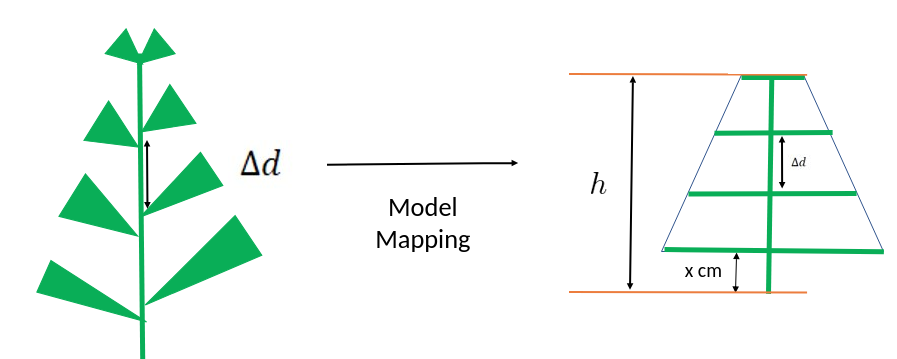
\includegraphics[width=0.9\textwidth,height=\textheight,keepaspectratio]{modelling/plant-model-3.png}
    \caption{Tomato plant model}
    \label{fig:plant:model:2}
\end{figure}

This model especially serves for the purpose of LAI calculation where the canopy visible from above can 
be mapped to the largest (and lowest) branch level of the plant - whereby each higher (and therefore newer)
level is smaller.
The size of the plant's entire leaf area is then correlated with the number of levels.
This model will be formalized in more detail later with all of its parameters. 